\documentclass[12pt]{beamer}

\usepackage{amsthm}
\usepackage[english]{babel}
\usepackage[utf8]{inputenc}

\usetheme{Copenhagen}

\title{The Hacker News Similarity Distance}
\author[Jacopo Notarstefano]{
    Jacopo Notarstefano\\
    \texttt{jacopo.notarstefano [at] gmail.com}
}
\date{10 February 2014}

\begin{document}
    \begin{frame}[plain]
        \titlepage
    \end{frame}

    \begin{frame}{Hacker News}
        \begin{figure}
            \centering
            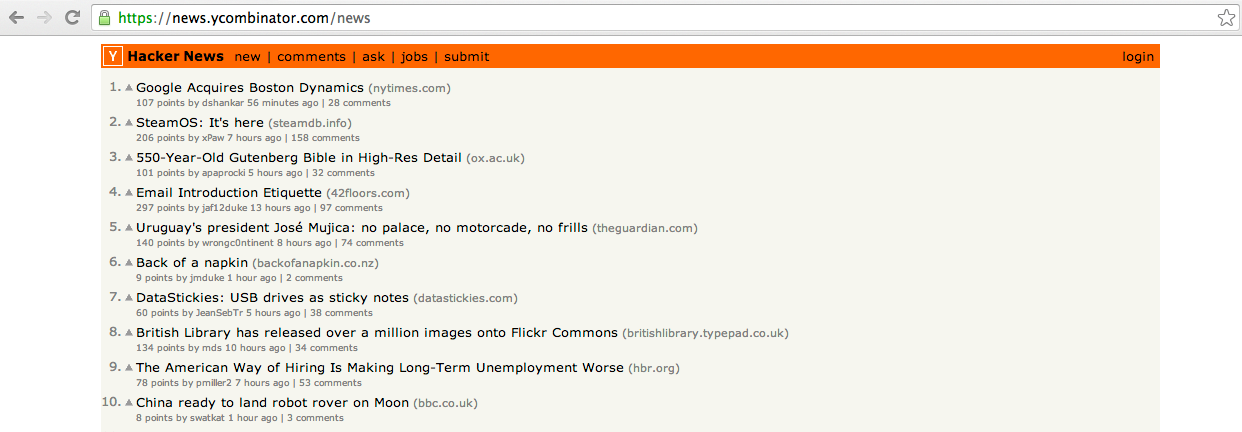
\includegraphics[width=\linewidth,keepaspectratio=true]{tex/img/hackernews.png}
        \end{figure}
    \end{frame}

    \begin{frame}{HNSearch}
        \begin{figure}
            \centering
            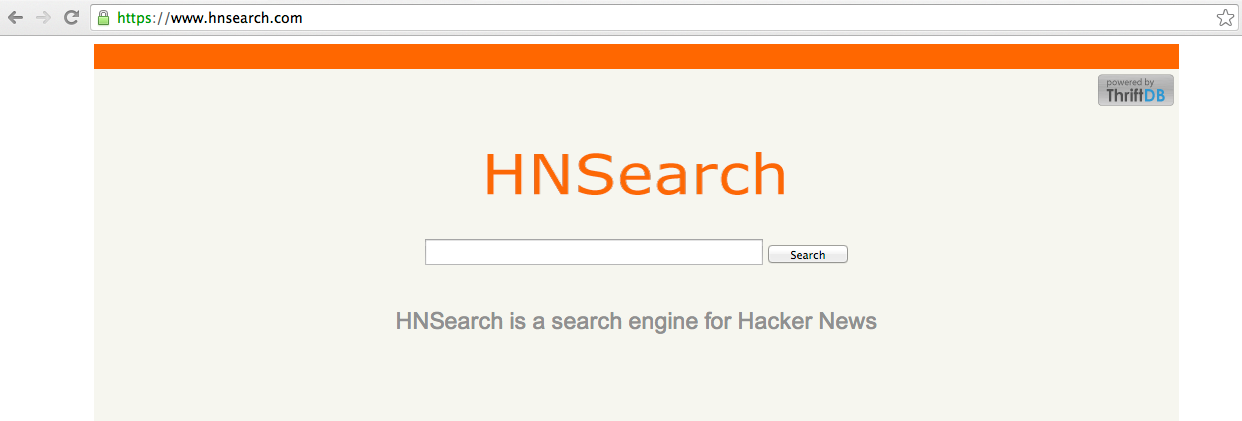
\includegraphics[width=\linewidth,keepaspectratio=true]{tex/img/hnsearch.png}
        \end{figure}
    \end{frame}

    \begin{frame}{ThriftDB}
        \begin{figure}
            \centering
            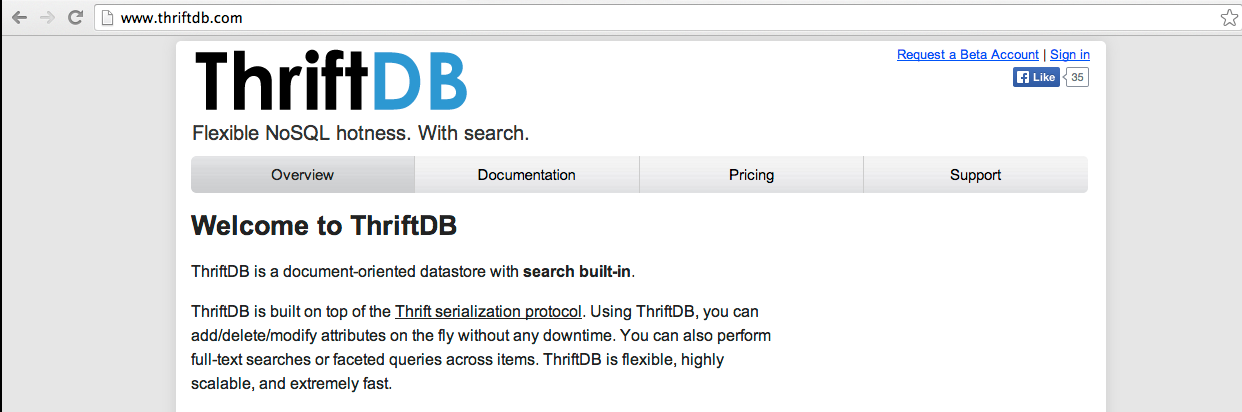
\includegraphics[width=\linewidth,keepaspectratio=true]{tex/img/thriftdb.png}
        \end{figure}
    \end{frame}

    \begin{frame}{A simple RESTful API}
    \end{frame}

    \begin{frame}{The Google Similarity Distance}
        \begin{definition}[Cilibrasi, Vit\'anyi 2007]
            Let \(x\) and \(y\) be search terms and \(N\) the size of the Google index. We define:
            \[
                \text{NGD}(x,y) = \frac{\max{\{\log{f(x)}, \log{f(y)}\}} - \log{f(x,y)}}{\log{N} - \min{\{\log{f(x)}, \log{f(y)}\}}}
            \]
            where \(f(x)\) denotes the number of pages containing \(x\), \(f(x,y)\) the number of pages containing both \(x\) and \(y\) as returned by Google.
        \end{definition}
    \end{frame}

    \begin{frame}{The Hacker News Similarity Distance}
        \begin{definition}
            Let \(x\) and \(y\) be search terms and \(N\) the size of the HNSearch index. We define:
            \[
                \text{NHND}(x,y) = \frac{\max{\{\log{f(x)}, \log{f(y)}\}} - \log{f(x,y)}}{\log{N} - \min{\{\log{f(x)}, \log{f(y)}\}}}
            \]
            where \(f(x)\) denotes the number of pages containing \(x\), \(f(x,y)\) the number of pages containing both \(x\) and \(y\) as returned by HNSearch.
        \end{definition}
    \end{frame}

    \begin{frame}{Implementation}
    \end{frame}

    \begin{frame}{Results}
    \end{frame}
\end{document}
